% Capítulo 4: decisão simples e decisão composta, lado a lado.
\documentclass[border=4pt]{standalone}
\usepackage[utf8]{inputenc}
\usepackage[T1]{fontenc}
% Estilo comum dos fluxogramas e diagramas de blocos.
\usepackage{tikz}
\usetikzlibrary{arrows.meta, positioning, calc, shapes.geometric, shapes.misc}
\definecolor{navy}{RGB}{23,45,80}
\definecolor{laranja}{RGB}{250,110,29}
\definecolor{cinzalogo}{RGB}{107,114,126}
\definecolor{azul}{RGB}{205,222,247}
\tikzset{
  base/.style={draw=navy, line width=0.9pt, font=\sffamily\small, align=center, inner sep=4pt},
  terminal/.style={base, rounded rectangle, fill=laranja!45, draw=laranja, minimum width=20mm, minimum height=7mm},
  processo/.style={base, rectangle, fill=laranja!12, minimum width=28mm, minimum height=8mm},
  decisao/.style={base, diamond, aspect=2.2, fill=azul, inner sep=1pt, minimum width=30mm},
  es/.style={base, trapezium, trapezium left angle=72, trapezium right angle=108,
             fill=white, minimum width=26mm, minimum height=8mm, trapezium stretches body},
  fluxo/.style={-{Stealth[length=2.2mm]}, navy, line width=0.9pt},
  rotulo/.style={font=\sffamily\small\bfseries, text=navy},
  legenda/.style={font=\sffamily\scriptsize, text=cinzalogo},
  resposta/.style={font=\sffamily\scriptsize\bfseries, text=navy},
}

\begin{document}
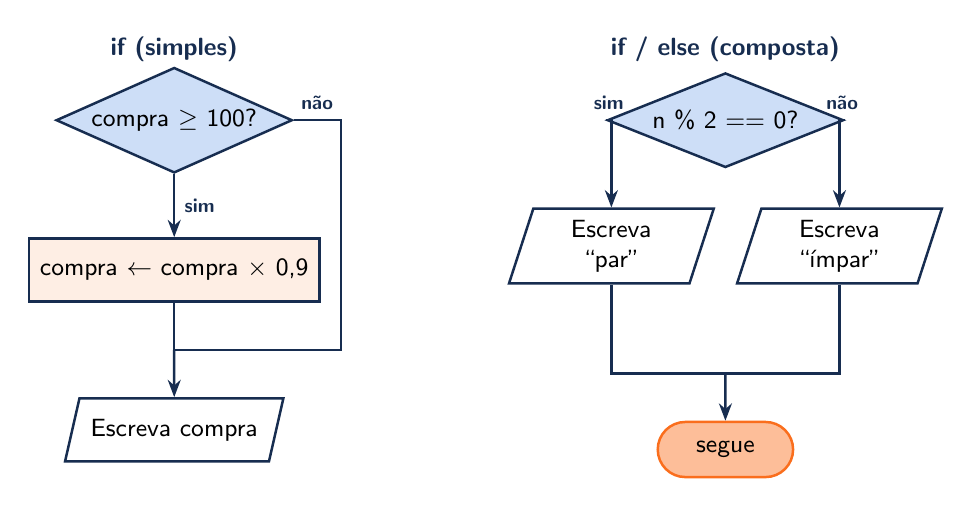
\begin{tikzpicture}[node distance=6mm]
  % simples
  \node[rotulo] (t1) at (0, 0.9) {if (simples)};
  \node[decisao] (d1) at (0, 0) {compra $\geq$ 100?};
  \node[processo, below=8mm of d1] (p1) {compra $\leftarrow$ compra $\times$ 0,9};
  \coordinate (j1) at ($(p1.south) + (0, -0.6)$);
  \node[es, below=6mm of j1] (s1) {Escreva compra};
  \draw[fluxo] (d1) -- node[resposta, right] {sim} (p1);
  \draw[navy, line width=0.9pt] (p1.south) -- (j1);
  \draw[navy, line width=0.9pt] (d1.east) -- ++(0.6, 0) node[resposta, above, pos=0.5] {não} |- (j1);
  \draw[fluxo] (j1) -- (s1);

  % composta
  \node[rotulo] (t2) at (7, 0.9) {if / else (composta)};
  \node[decisao] (d2) at (7, 0) {n \% 2 == 0?};
  \node[es, below left=8mm and 2mm of d2] (a2) {Escreva\\``par''};
  \node[es, below right=8mm and 2mm of d2] (b2) {Escreva\\``ímpar''};
  \coordinate (j2) at ($(d2.south) + (0, -2.6)$);
  \node[terminal, below=6mm of j2] (f2) {segue};
  \draw[fluxo] (d2.west) -| node[resposta, above, pos=0.25] {sim} (a2.north);
  \draw[fluxo] (d2.east) -| node[resposta, above, pos=0.25] {não} (b2.north);
  \draw[navy, line width=0.9pt] (a2.south) |- (j2);
  \draw[navy, line width=0.9pt] (b2.south) |- (j2);
  \draw[fluxo] (j2) -- (f2);
\end{tikzpicture}
\end{document}
